\begin{figure*}
    \centering
    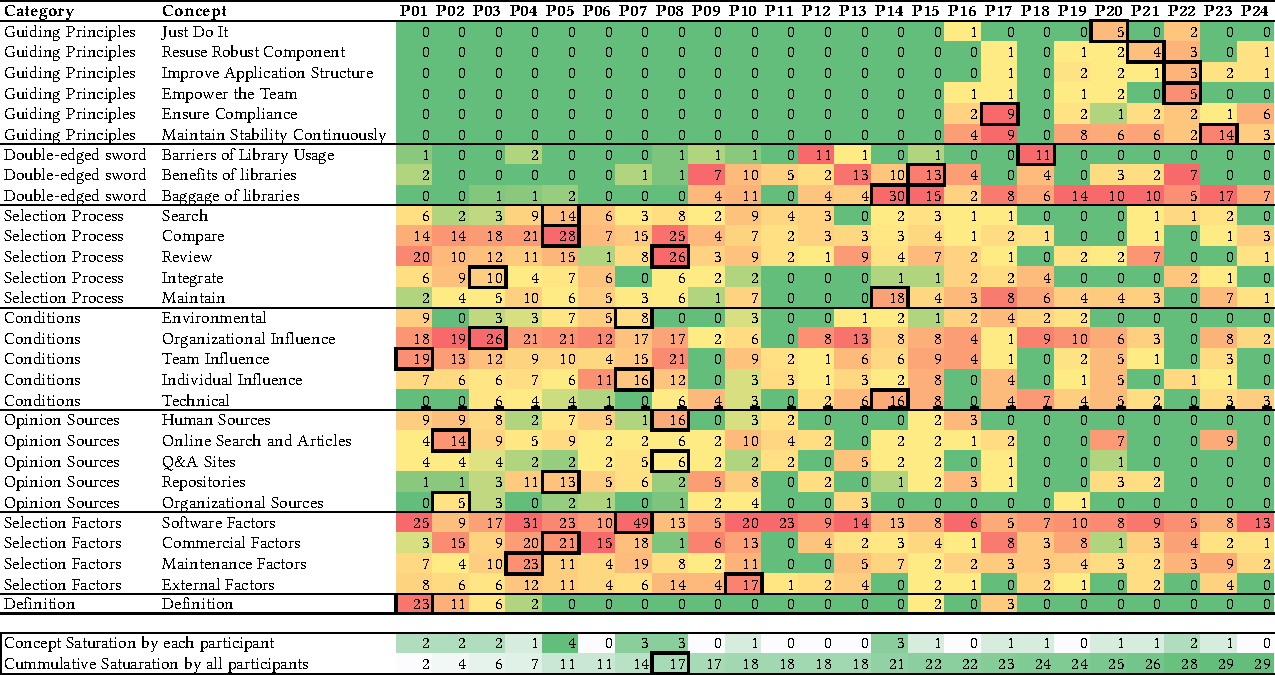
\includegraphics[scale=0.85]{images/saturation.pdf}
    \caption{Heatmap of concept saturation over the interviews. Red refers to higher discussion of a concept by an interviewee, the number refers to how many times interviewee has discussed a concept. Green refers to lower discussion of concepts by an interviewee. Thick black bordered cells refer to the most discussion reference of a concept among all participants. For example, review concept under selection process category was discussed 26 times in P08's interview and hence the corresponding cell is marked by thick border.}
    \label{fig:saturation}
\end{figure*}